\documentclass[a4paper, conference]{IEEEtran} %changed paper style to A4. MB
\IEEEoverridecommandlockouts
% Following line is added by Mert Biricik (MB). It is for quoting text by \enquote{} command.
\usepackage [autostyle, english = british]{csquotes}
% The preceding line is only needed to identify funding in the first footnote. If that is unneeded, please comment it out.
\usepackage{cite}
\usepackage{amsmath,amssymb,amsfonts}
\usepackage{algorithmic}
\usepackage{graphicx}
\usepackage{textcomp}
\usepackage{xcolor}
\def\BibTeX{{\rm B\kern-.05em{\sc i\kern-.025em b}\kern-.08em
    T\kern-.1667em\lower.7ex\hbox{E}\kern-.125emX}}
\begin{document}

\title{DataTürk Project\\
{\footnotesize \textsuperscript{}}
\thanks{}
}
% Authors are sorted by surnames. MB
\author{\IEEEauthorblockN{1\textsuperscript{st} Mert Biricik}
\IEEEauthorblockA{\textit{Management Information Systems} \\
\textit{Kadir Has University}\\
Istanbul, Turkey \\
mertbiricik@stu.khas.edu.tr}
\and
\IEEEauthorblockN{2\textsuperscript{nd} Beril Elçin Bülbül}
\IEEEauthorblockA{\textit{Management Information Systems} \\
\textit{Kadir Has University}\\
Istanbul, Turkey \\
belcin.bulbul@stu.khas.edu.tr}
\and
\IEEEauthorblockN{3\textsuperscript{rd} Hasan Coşkun}
\IEEEauthorblockA{\textit{Management Information Systems} \\
\textit{Kadir Has University}\\
Istanbul, Turkey \\
hasan.coskun@stu.khas.edu.tr}
\and
\IEEEauthorblockN{4\textsuperscript{th} Beril Kurt}
\IEEEauthorblockA{\textit{Management Information Systems} \\
\textit{Kadir Has University}\\
Istanbul, Turkey \\
beril.kurt@stu.khas.edu.tr}
\and
\IEEEauthorblockN{5\textsuperscript{th} Sude Kulbay}
\IEEEauthorblockA{\textit{Management Information Systems} \\
\textit{Kadir Has University}\\
Istanbul, Turkey \\
sudekulbay@stu.khas.edu.tr}
\and
\IEEEauthorblockN{6\textsuperscript{th} Emir Şahin}
\IEEEauthorblockA{\textit{Management Information Systems} \\
\textit{Kadir Has University}\\
Istanbul, Turkey \\
esad.emir34@stu.khas.edu.tr}
}

\maketitle

\begin{abstract}
This document is the first progress report for DataTürk's machine learning project.
The document contains the details of the dataset cleansing process.
\end{abstract}

\begin{IEEEkeywords}
machine learning, github, dataset, missing values, graphs
\end{IEEEkeywords}

\section{Introduction}
We created a python script, which can be found on our repo\cite{datatürk}, to identify the missing values in our given dataset, and
analyze the data according to their contextual meaning.
\section{Data Preprocessing}

\subsection{Dropping Some of the Columns and Filling the Values}

We identified the columns that contained more than 50 percent of the missing data values in them and filled in the missing values in these numeric columns using the calculated mean of such columns.
For non-numeric columns we used the mode.

\subsection{Creating a Binary Label for the Data}
We converted the last columnt to a binary label column. 
\subsection{Summary of the Dataset}

Total number of missing values in the DataFrame: 0 \\
\indent Total number of missing values in binary label column: 0\\
\indent Non-numerical columns number is: 13\\
\indent Numerical columns number is: 68\\
\indent Total number of rows in the DataFrame: 246008\\
\indent Total number of columns in the DataFrame: 81

\begin{figure}
\graphicspath{ {./images/} }
\centerline{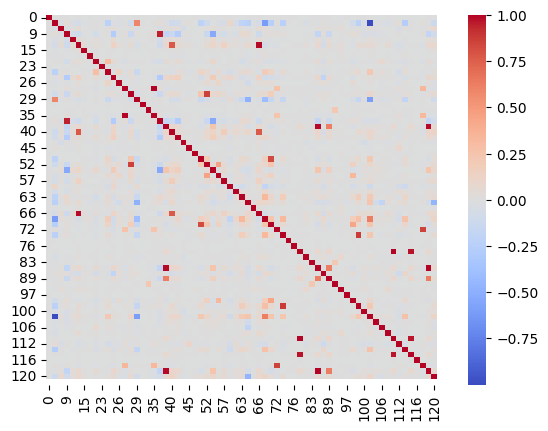
\includegraphics[scale=.65]{dataset}}
\caption[short]{Correlation between information on the dataset.}
\label{graph}
\end{figure}

\begin{figure}
\graphicspath{ {./images/} }
\centerline{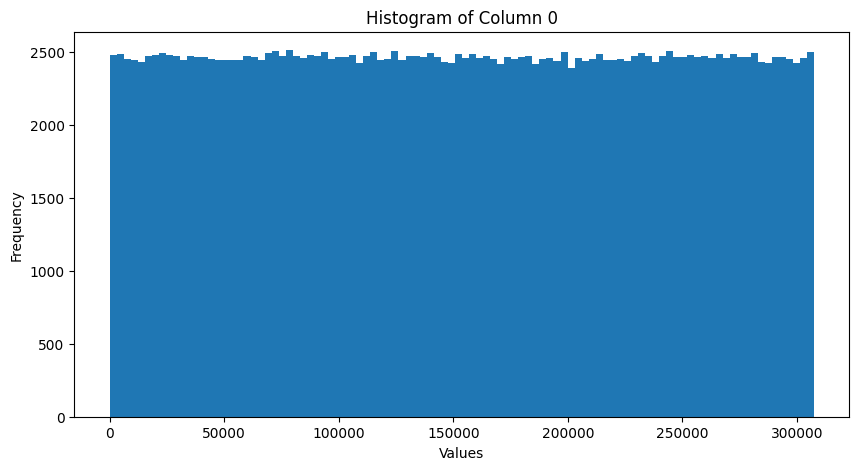
\includegraphics[scale=.42]{dataset2}}
\caption[short]{Correlation between information on the dataset.}
\label{graph2}
\end{figure}
\pagebreak
\section{Application of Classical Data Science Techniques}

% This bibliography style is added afterwards by MB for easier citation.
\bibliographystyle{IEEEtran}
\flushleft
\bibliography{IEEEabrv, bibliography.bib}


% This part is not needed but didn't want to delete. MB

%\begin{thebibliography}{00}
%\bibitem{b1} G. Eason, B. Noble, and I. N. Sneddon, ``On certain integrals of Lipschitz-Hankel type involving products of Bessel functions,'' Phil. Trans. Roy. Soc. London, vol. A247, pp. 529--551, April 1955.
%\bibitem{b2} J. Clerk Maxwell, A Treatise on Electricity and Magnetism, 3rd ed., vol. 2. Oxford: Clarendon, 1892, pp.68--73.
%\bibitem{b3} I. S. Jacobs and C. P. Bean, ``Fine particles, thin films and exchange anisotropy,'' in Magnetism, vol. III, G. T. Rado and H. Suhl, Eds. New York: Academic, 1963, pp. 271--350.
%\bibitem{b4} K. Elissa, ``Title of paper if known,'' unpublished.
%\bibitem{b5} R. Nicole, ``Title of paper with only first word capitalized,'' J. Name Stand. Abbrev., in press.
%\bibitem{b6} Y. Yorozu, M. Hirano, K. Oka, and Y. Tagawa, ``Electron spectroscopy studies on magneto-optical media and plastic substrate interface,'' IEEE Transl. J. Magn. Japan, vol. 2, pp. 740--741, August 1987 [Digests 9th Annual Conf. Magnetics Japan, p. 301, 1982].
%\bibitem{b7} M. Young, The Technical Writer's Handbook. Mill Valley, CA: University Science, 1989.
%\end{thebibliography}

\end{document}
